\documentclass[conference]{IEEEtran}
% \IEEEoverridecommandlockouts  % only needed for a funding footnote; none here
\usepackage{cite}
\usepackage{amsmath,amssymb,amsfonts}
\usepackage{graphicx}
\usepackage{textcomp}
\usepackage{booktabs}
% No character protrusion: it pushes line-end punctuation into the column gutter,
% which EDAS measures (minimum 0.12 in).
\usepackage[protrusion=false]{microtype}
\usepackage{tikz}
\usetikzlibrary{arrows.meta,positioning,calc}

\graphicspath{{figures/}}

\newcommand{\SN}{R}            % signal-to-noise power ratio, S/N
\newcommand{\dB}{~dB}
\newcommand{\Nin}{N_\mathrm{in}}

\begin{document}

\title{One Layer, Eight Inputs, Two Bits: The Price of Fidelity in Spiking
Biosignal Processors}

\author{\IEEEauthorblockN{Ahad Ulla Baig}
\IEEEauthorblockA{\textit{Dept. of Artificial Intelligence} \\
\textit{and Machine Learning} \\
\textit{Ramaiah Institute of Technology}\\
Bengaluru, India \\
ahadullabaig.16@gmail.com}
\and
\IEEEauthorblockN{Divisha Gera}
\IEEEauthorblockA{\textit{Dept. of Artificial Intelligence} \\
\textit{and Machine Learning} \\
\textit{Ramaiah Institute of Technology}\\
Bengaluru, India \\
divisha.018@gmail.com}
\and
\IEEEauthorblockN{Charithra G}
\IEEEauthorblockA{\textit{Dept. of Artificial Intelligence} \\
\textit{and Machine Learning} \\
\textit{Ramaiah Institute of Technology}\\
Bengaluru, India \\
charithra754@gmail.com}
}

\maketitle

\begin{abstract}
Neuromorphic processors pay for a spiking neural network per synaptic
operation, per routed spike and per stored weight bit, yet the fidelity a
spiking signal chain delivers is seldom weighed against those costs. We
simulate rate-coded leaky integrate-and-fire networks that reconstruct
biosignals and attach a hardware cost to about 200 design points on the
MIT-BIH arrhythmia database. Every design on the cost--fidelity fronts is a
single spiking layer; a second layer costs 2.5 times the synaptic work and
0.9 dB of fidelity. With each neuron limited to eight inputs, widening the pool
of input spike trains raises fidelity at no cost in synaptic operations, and a
spike-counting term predicts the fidelity cost of a slower encoder to within
0.07 dB. One layer of 128 neurons, each reading 8 of 512 input channels, is
statistically equivalent to the best design we had measured, with one eighth
of its synaptic operations and synapses and three quarters of its spikes. This
holds on ECG windows no earlier experiment used and at noisy inputs, and the
design is no worse on a synthetic EEG and a sine. It keeps its fidelity with
2-bit weights, loses at most 0.22 dB with 1-bit weights, and loses at most
0.69 dB when three quarters of its synaptic devices are stuck at zero. A
break-even condition on the ratio of spike energy to synaptic-operation energy
tells a designer when to spend one to save the other.
\end{abstract}

\begin{IEEEkeywords}
spiking neural networks, neuromorphic hardware, synaptic operations,
address-event representation, weight quantization, device variation, ECG
\end{IEEEkeywords}

\section{Introduction}

A neuromorphic processor does work when a spike arrives: it reads a weight for
every synapse the spike reaches, updates the neurons it drives, and routes any
spike they emit~\cite{davies2018loihi}. Sparsity in activity and in
connectivity is therefore a central lever on the hardware efficiency of spiking
neural networks (SNNs)~\cite{aliyev2024sparsity}, and synaptic operations are a
common proxy for their energy~\cite{sorbaro2020energy}. For an always-on
biosignal processor, the question an architect faces is concrete: what does
each decibel of signal fidelity cost in synaptic operations, spikes and weight
memory, and which design choices buy it most cheaply?

Earlier, we reported that feed-forward networks of leaky integrate-and-fire
(LIF) neurons that reconstruct a biosignal from rate-coded spikes reach a
fidelity \emph{ceiling}~\cite{baig2026icee}. Their output
signal-to-noise ratio (SNR) stops improving as the input improves; a cascade
law in the form of Friis's noise formula~\cite{friis1944noise} predicts the
ceiling; noise that neurons share sets it; and giving each neuron a fixed
fan-in of 8--16 inputs raises it. That work measured fidelity only. Here we
attach hardware costs to every design point, add two levers the earlier grids
never varied, and test the designs that come out on data held back for the
purpose. Our contributions are:
\begin{itemize}
\item \emph{A cost--fidelity landscape} for spiking signal chains
(Section~\ref{sec:landscape}). Every design on the synaptic-operation and
spike fronts is a single LIF layer. Past that choice, fidelity costs about
0.2\dB{} per doubling of synaptic work.
\item \emph{Two cheap levers} (Section~\ref{sec:pool}). At fixed fan-in, a
wider pool of input spike trains raises the ceiling by 0.2--0.3\dB{} per
doubling without adding synaptic operations. A spike-counting term in the
cascade law prices the encoder rate to 0.07\dB.
\item \emph{A confirmed design} (Section~\ref{sec:designs}). One layer of 128
neurons with 8 inputs each from a 512-channel pool matches the previous best
design within $\pm0.5$\dB{} at one eighth of the synaptic operations, with
2-bit weights, on unseen ECG and at noisy inputs, and is no worse on two
further signals. A
break-even ratio tells when trading synaptic operations for spikes pays.
\item \emph{A precision and fault budget} (Section~\ref{sec:devices}). One-bit
weights cost at most 0.22\dB, and a quarter of devices stuck at zero at most
0.15\dB. A model based on effective fan-in ranks these losses correctly but
overstates their size about twofold.
\end{itemize}

\section{Background and Related Work}

\emph{Costs of spiking hardware.} Event-driven processors spend energy per
synaptic operation and per spike~\cite{davies2018loihi,sorbaro2020energy}.
Spikes travel between cores as address events, packets of $\log_2 N$ bits that
name one of $N$ neurons~\cite{boahen2000aer}, so spike traffic is a cost in its
own right, and lossy compression of that traffic has been proposed to reduce
it~\cite{ganesh2025fspc}. Moving weights and state through a memory hierarchy is
another~\cite{chee2025profiling}. We count synaptic operations, spikes and
weight bits, and leave their energies as parameters, since they differ between
chips.

\emph{Device non-idealities.} Emerging nonvolatile synapses suffer
device-to-device variation~\cite{yu2018nvm}. In resistive crossbars,
resistance variation and stuck-at faults degrade the accuracy of neural
networks~\cite{chen2017rram}, and conductances cannot be negative, so signed
weights take pairs of devices~\cite{prezioso2015training}. Low-precision
weights reduce memory and energy in SNNs trained for
recognition~\cite{rathi2019stdp,putra2021qspinn}. These studies measure
classification accuracy. We measure how faithfully a continuous signal
survives, for which there is no accuracy to fall back on.

\emph{Spiking biosignal processing.} Spike encodings of MIT-BIH ECG have been
used for lightweight beat classification~\cite{sulistiyanto2025ecg}.
Reconstruction is a different task: the output must follow the waveform. For
the rate-coded networks studied here, fidelity is bounded by shared noise, as
correlated noise bounds the information a neural population
carries~\cite{morenobote2014information}, and the bound can be designed
against~\cite{baig2026icee}.

\section{System and Cost Model}
\label{sec:model}

\begin{figure}[t]
\centering
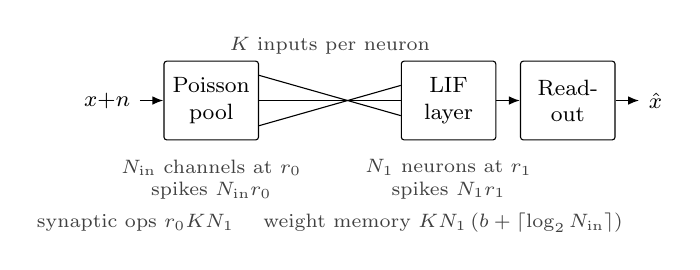
\begin{tikzpicture}[
  font=\footnotesize,
  blk/.style={draw, rounded corners=1pt, minimum height=10mm,
    minimum width=12mm, align=center, inner sep=2pt},
  arr/.style={-{Latex[length=1.4mm,width=1.1mm]}, semithick},
  cost/.style={font=\scriptsize, align=center, text=black!75}]
\node (x) {$x{+}n$};
\node[blk, right=3mm of x] (pool) {Poisson\\pool};
\node[blk, right=18mm of pool] (lif) {LIF\\layer};
\node[blk, right=3mm of lif] (ro) {Read-\\out};
\node[right=3mm of ro] (xh) {$\hat{x}$};
\draw[arr] (x) -- (pool);
\foreach \dy in {-3.2mm, 0mm, 3.2mm} {
  \draw[thin] ($(pool.east)+(0,\dy)$) -- ($(lif.west)+(0,{-0.6*\dy})$);
}
\draw[arr] (lif) -- (ro);
\draw[arr] (ro) -- (xh);
\node[cost] at ($(pool)!0.5!(lif)+(0,7mm)$) {$K$ inputs per neuron};
\node[below=1.2mm of pool, cost] {$\Nin$ channels at $r_0$\\spikes $\Nin r_0$};
\node[below=1.2mm of lif, cost] {$N_1$ neurons at $r_1$\\spikes $N_1 r_1$};
\node[cost] at ($(pool)!0.5!(lif)+(0,-15.5mm)$)
  {synaptic ops $r_0 K N_1$ \quad
   weight memory $K N_1\,(b + \lceil\log_2 \Nin\rceil)$};
\end{tikzpicture}
\caption{The one-layer signal chain and what it costs per second. A noisy
signal drives a pool of $\Nin$ Poisson channels at rate $r_0$; each of $N_1$ LIF
neurons reads $K$ of them; a causal population readout returns $\hat{x}$. At a
fixed fan-in, synaptic work does not depend on the pool width.}
\label{fig:pipeline}
\end{figure}

\subsection{The signal chain}
A signal sampled at 250~Hz (4~ms steps) drives $\Nin$ Poisson channels. Each
fires with probability proportional to the signal's amplitude normalized to the
drive's own range, so the channels carry the same signal with independent
counting noise; we call them the \emph{input pool}. LIF neurons (rest
$-70$~mV, threshold $-55$~mV, reset $-80$~mV, membrane time constant 20~ms,
refractory period 2~ms) integrate weighted input spikes. In a fixed-fan-in
layer each neuron reads exactly $K$ channels chosen at random, with weights
uniform on $[0,1]$; dense layers read every channel, with weights uniform on
$[0, 0.3]$. The output is the mean of
the output neurons' exponentially filtered spike trains (time constant 20~ms),
a causal readout. The networks are untrained. The encoder's maximum rate and
each layer's gain are bisected until the encoder and every layer fire at their
target rates, $r_0$ and $r_1$, a form of the rate normalization used to convert
networks to spikes~\cite{diehl2015balancing,rueckauer2017conversion}. We write
networks as their widths, input pool first: $[512,128]$ is a 512-channel pool
and one layer of 128 neurons.

\subsection{Hardware cost}
For a network of widths $N_0 = \Nin, N_1, \dots, N_L$ with mean rates
$r_0, \dots, r_L$, where layer $k$ has $S_k$ synapses ($K N_k$ at a fixed fan-in,
$N_{k-1} N_k$ when dense), the costs per second are
\begin{align}
O &= \sum_{k=1}^{L} r_{k-1} S_k, \qquad
E = \sum_{k=0}^{L} N_k r_k, \label{eq:cost}\\
M &= \sum_{k=1}^{L} S_k \bigl(b + a_k\bigr),
\label{eq:memory}
\end{align}
where $O$ counts synaptic operations, the work of an event-driven
chip~\cite{sorbaro2020energy}; $E$ counts spikes, including the encoder's, as
address events to route~\cite{boahen2000aer}; and $M$ counts the bits of $b$-bit
weights plus, for a fixed-fan-in layer, an $a_k = \lceil \log_2 N_{k-1}
\rceil$-bit input address per synapse (a dense crossbar indexes by position,
so $a_k = 0$). A clock-driven implementation instead reads every synapse and
updates every neuron at every 4~ms step, $250 \sum_k S_k$ reads and $250
\sum_{k \ge 1} N_k$ updates per second, whatever the rates. We compute $O$ and
$E$ from each run's measured rates.

\subsection{Fidelity and its budget}
A readout's gain and offset are arbitrary, so fidelity is the affine-corrected
SNR: $\hat{x}$ is regressed onto the clean signal $x$ and scored as
$\mathrm{var}(x)/\mathrm{var}(x - \hat{x})$. For signal plus independent noise
this equals $1 + \SN$, with $\SN$ the signal-to-noise power ratio. The
\emph{ceiling} $C$ is the output SNR at a noiseless input. Inverse S/N adds
along the chain~\cite{baig2026icee},
\begin{equation}
\frac{1}{\SN_\mathrm{out}} = \frac{1}{\SN_\mathrm{in}} + \sum_k
\frac{1}{\Lambda_k},
\label{eq:law}
\end{equation}
where $\Lambda_k$ is stage $k$'s intrinsic S/N. Poisson counting noise has a
variance proportional to the rate, so the encoder's share of the sum should
scale as $1/r_0$. At a noiseless input this splits the ceiling into a part the
encoder rate buys and a remainder it cannot:
\begin{equation}
\frac{1}{\SN_C} = \frac{c}{r_0} + \frac{1}{\Lambda_\mathrm{rest}},
\label{eq:budget}
\end{equation}
with $c$ and $\Lambda_\mathrm{rest}$ fixed by the network and the signal.

\begin{figure*}[t]
\centering
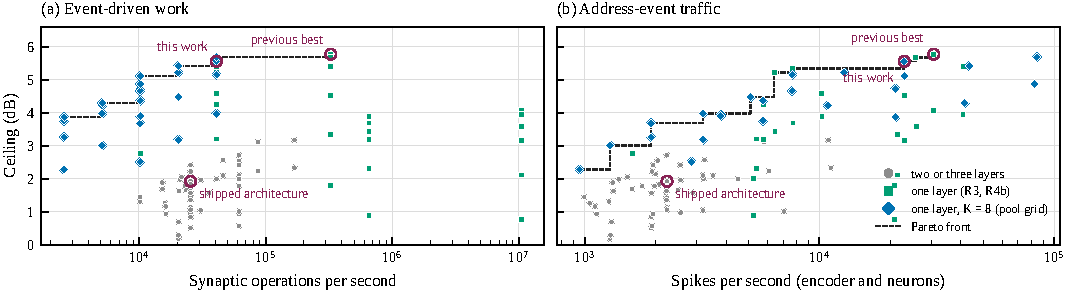
\includegraphics[width=\textwidth]{fig_landscape.pdf}
\caption{Ceiling against (a) synaptic operations and (b) spikes per second for
100 exact-weight designs on MIT-BIH, medians over records (seeds 0--9 or 0--4).
Grey: two or three LIF layers; green: one layer from the earlier grids; blue:
the pool grid. Dashed: the Pareto front. Circled: the reference $[32,16,8]$
network, the previous best $[512,512]$ with $K = 16$, and the $[512,128]$
design with $K = 8$ of Section~\ref{sec:designs}.}
\label{fig:landscape}
\end{figure*}

\begin{table}[t]
\centering
\caption{What each lever buys and costs on MIT-BIH}
\label{tab:levers}
\scriptsize
\setlength{\tabcolsep}{3pt}
\begin{tabular}{@{}lccc@{}}
\toprule
Change & $\Delta$ceiling, dB [95\% CI] & Synops & Spikes \\
\midrule
Second LIF layer, $[32,8]\to[32,16,8]$ & $-$0.91 [$-$1.09, $-$0.79] & 2.50 & 1.40 \\
Third LIF layer & $-$0.36 [$-$0.40, $-$0.30] & 1.40 & 1.29 \\
10 STDP epochs, rates held & $-$0.49 [$-$0.60, $-$0.39] & 1.00 & 1.00 \\
Output rate 40 $\to$ 5 Hz & +0.65 [+0.02, +1.27] & 1.00 & 0.87 \\
Output width 8 $\to$ 64 & +0.08 [+0.06, +0.09] & 2.41 & 2.00 \\
Input width 32 $\to$ 256, dense & +0.45 [+0.33, +0.56] & 6.61 & 5.00 \\
Fan-in dense $\to$ 16, $[512,512]$ & +1.85 [+1.38, +2.26] & 0.031 & 1.00 \\
Input pool 128 $\to$ 2048, $K=8$ & +0.57 [+0.28, +0.90] & 1.00 & 11.0 \\
Encoder 40 $\to$ 10 Hz, $[128,128]$ & $-$1.29 [$-$1.65, $-$0.85] & 0.25 & 0.50 \\
\bottomrule
\end{tabular}

\vspace{2pt}
\parbox{\columnwidth}{\scriptsize Paired by record ($n=16$), noiseless input; cost columns are ratios after/before. Rows 1--7 from the earlier grids, rows 8--9 from the pool grid.}
\end{table}

\begin{table*}[t]
\centering
\caption{The named designs, re-measured on unseen data}
\label{tab:designs}
\footnotesize
\setlength{\tabcolsep}{4.5pt}
\begin{tabular}{@{}llcccccc rrrrr@{}}
\toprule
 & & & Enc. & Weight & \multicolumn{3}{c}{Ceiling (dB)} & \multicolumn{2}{c}{Event-driven} & \multicolumn{3}{c}{Static} \\
\cmidrule(lr){6-8}\cmidrule(lr){9-10}\cmidrule(l){11-13}
 & Network & Fan-in & (Hz) & bits & MIT-BIH & EEG & Sine & Synops & Spikes & Synapses & Memory & Clock \\
\midrule
D0 & $[32,16,8]$ & all & 40 & -- & 1.72 & 2.03 & 7.52 & 25.6 & 2.2 & 640 & 20.5 & 160 \\
D1 & $[512,512]$ & 16 & 40 & -- & 6.08 & 3.24 & 12.18 & 327.7 & 30.8 & 8,192 & 335.9 & 2,048 \\
D2 & $[512,128]$ & 8 & 40 & -- & 5.94 & 3.11 & 12.35 & 41.0 & 23.1 & 1,024 & 42.0 & 256 \\
D3 & $[512,128]$ & 8 & 40 & 2 & 5.94 & 3.13 & 12.39 & 41.0 & 23.1 & 1,024 & 11.3 & 256 \\
D4 & $[2048,128]$ & 8 & 10 & -- & 5.35 & 2.97 & 12.26 & 10.2 & 23.0 & 1,024 & 44.0 & 256 \\
D5 & $[128,128]$ & 8 & 40 & -- & 5.44 & 3.06 & 11.87 & 41.0 & 7.7 & 1,024 & 39.9 & 256 \\
\bottomrule
\end{tabular}

\vspace{2pt}
{\scriptsize D2 minus D1 $-$0.23 [$-$0.45, +0.02]~dB; D3 minus D2 0.00 [$-$0.02, +0.01]; D4 minus D5 $-$0.06 [$-$0.12, +0.04]. Medians over 16 records (MIT-BIH) or 10 seeds, seeds 10--19, noiseless input. Synops and spikes: thousands per second, measured. Memory: kilobits of weights, at 32 bits unless quantized, plus an input address per synapse of a fixed-fan-in layer. Clock: thousands of synapse reads per second at 250 steps per second.}
\end{table*}


\section{Experimental Method}
\label{sec:method}

\emph{Signals.} Real ECG comes from 16 records of the MIT-BIH Arrhythmia
Database~\cite{moody2001impact,goldberger2000physionet}. Each random seed
selects a different artifact-free 10~s window, resampled to 250~Hz. We add a
synthetic electroencephalogram (EEG) with 10, 20 and 40~Hz components of
random phase, and a 2~Hz sine. Gaussian noise is scaled so that the input SNR
equals its nominal value exactly.

\emph{Grids.} The landscape combines 76 MIT-BIH design points from our earlier
grids~\cite{baig2026icee}, covering depth, width, output rate, training and fan-in, with a
\emph{pool grid} of 24 one-layer designs: $K = 8$, $N_1 \in \{32, 128\}$,
$\Nin \in \{32, 128, 512, 2048\}$, $r_0 \in \{10, 20, 40\}$~Hz and $r_1 = 20$~Hz
(1,920 runs). A \emph{device grid} applies one non-ideality at a time to the
three $N_1 = 128$ pools at all three encoder rates (8,640 runs), after the
weights are programmed and before rates are calibrated. The non-idealities
are quantization to $2^b$ evenly spaced levels on $[0, \max w]$; lognormal
device-to-device variation, $w \mapsto w\,e^{\sigma z}$ with $z \sim
\mathcal{N}(0,1)$; and stuck-at-zero devices. A \emph{confirmation grid}
re-measures six named designs (Table~\ref{tab:designs}) on seeds 10--19 (3,240
runs). On MIT-BIH these select windows no earlier grid used; every record has
at least 103 clean windows. It uses noiseless, 10\dB{} and 0\dB{} inputs on
MIT-BIH, EEG and the sine. Earlier grids used 10 seeds, and the pool and device
grids used seeds 0--4.

\emph{Statistics.} The unit of analysis is a record ($n = 16$) or, for
synthetic signals, a seed ($n = 10$). SNRs average a unit's runs. Paired
comparisons report the median difference with a bias-corrected and
accelerated (BCa) bootstrap 95\% interval and the Wilcoxon signed-rank test,
with Holm correction within families. Equivalence uses two one-sided tests at
$\pm0.5$\dB. The tests and decision rules of the pool, device and confirmation
grids were written into their scripts before each grid ran, and those of the
device and confirmation grids, with the device grid's numeric predictions, were
committed to version control first; analyses designed after seeing data are
marked post hoc. Cells shared between grids
reproduce exactly (80 and 720 runs).

\section{Results}

\subsection{The cost--fidelity landscape}
\label{sec:landscape}

Fig.~\ref{fig:landscape} places every design on two cost axes. Every point on
both Pareto fronts is a single LIF layer. The reference two-layer network,
$[32,16,8]$ with every stage at 40~Hz, reaches 1.92\dB{} for $2.6\times10^4$
synaptic operations per second; removing its hidden layer gains 0.91\dB{} and
cuts synaptic work by a factor of 2.5 (Table~\ref{tab:levers}). Depth costs
twice, in work and in fidelity, as~\eqref{eq:law} requires: each spiking stage
adds its own term.

Beyond depth, the levers price very differently. Widening a dense input layer
eightfold buys 0.45\dB{} for 6.6 times the synaptic work, about 0.2\dB{} per
doubling. Widening a fixed-fan-in layer from $[128,128]$ with $K = 8$ to
$[512,512]$ with $K = 16$ buys the same rate, 0.21\dB{} per doubling. Fixing
fan-in is the one change in Table~\ref{tab:levers} that raises fidelity and
cuts cost together. The output rate is the largest operating-point lever
($+0.65$\dB{} at 5~Hz) but moves almost no synaptic work: the encoder's spikes
into the first layer account for 80\% of the synaptic operations in
$[32,16,8]$ and all of them in a one-layer network, while output spikes feed
only the readout.

\subsection{Input pool and encoder rate}
\label{sec:pool}

\begin{figure}[t]
\centering
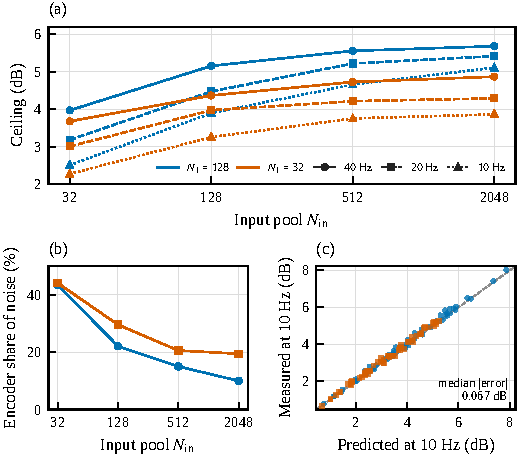
\includegraphics[width=\columnwidth]{fig_pool.pdf}
\caption{Pool grid, MIT-BIH, $K = 8$, layer at 20~Hz. (a) Ceiling against
input pool width for two layer widths and three encoder rates; medians over
16 records. (b) Share of output noise due to encoder counting at 40~Hz, from
\eqref{eq:budget} fitted at 20 and 40~Hz (post hoc). (c) The 10~Hz ceiling
predicted by \eqref{eq:budget} from the 20 and 40~Hz ceilings against the
measured one, per record and architecture (128 cells); dashed, identity.}
\label{fig:pool}
\end{figure}

At a fixed fan-in, the synaptic work of a layer is $r_0 K N_1$ whatever the
pool width, while a wider pool lowers the overlap between the inputs that
different neurons read. The ceiling rises with the pool at every encoder rate
(Fig.~\ref{fig:pool}a): by $+0.20$ [$+0.12$, $+0.29$]\dB{} per doubling at
$N_1 = 32$ and $+0.29$ [$+0.15$, $+0.42$] at $N_1 = 128$ (Holm-adjusted
$p = 6\times10^{-5}$ for both). From 128 to 2048 channels at $N_1 = 128$ it
gains $+0.57$ [$+0.28$, $+0.90$]\dB. The cost moves to address events: the
pool's spikes grow as $\Nin r_0$.

Slowing the encoder halves synaptic work per halving of $r_0$ and costs
0.34--0.80\dB{} per halving, significantly at all eight architectures, least
with the widest pool. The budget~\eqref{eq:budget} prices this. Fitted to each
record's ceilings at 20 and 40~Hz, it predicts the 10~Hz ceiling with a median
absolute error of 0.067\dB{} (90th percentile 0.20\dB) over 128
record--architecture cells spanning 0.7 to 8.0\dB{} (Fig.~\ref{fig:pool}c). Encoder counting noise is 44\% of the output noise
with a 32-channel pool and 10\% with 2048 channels (Fig.~\ref{fig:pool}b), and
the remainder $\Lambda_\mathrm{rest}$, the layer's own shared error, barely
moves: 5.6 to 6.1\dB{} at $N_1 = 128$. A wide pool makes the encoder rate
cheap to cut; nothing in the input budget lifts a $K = 8$ layer much past
6\dB{} on ECG.

\subsection{The named designs on unseen data}
\label{sec:designs}

\begin{figure}[t]
\centering
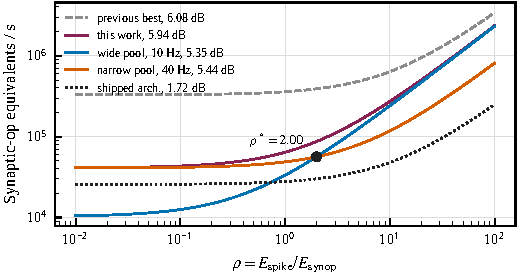
\includegraphics[width=\columnwidth]{fig_break_even.pdf}
\caption{Event cost of the confirmation designs, $O + \rho E$ in
synaptic-operation equivalents, against the ratio $\rho$ of spike to
synaptic-operation energy (MIT-BIH, noiseless input). The wide pool with a slow
encoder is cheaper than the narrow pool with a fast one below
$\rho^* = 2.00$, at the same fidelity.}
\label{fig:breakeven}
\end{figure}

The landscape suggested a design, $[512,128]$ with $K = 8$ and a 40~Hz encoder,
that matches the previous best, $[512,512]$ with $K = 16$, at far lower cost. That
comparison was made after seeing the data, and on different seeds for the two
designs, so we re-measured six designs on held-out data
(Table~\ref{tab:designs}). All tests committed in advance held.
\begin{itemize}
\item \emph{Matching the best.} D2 minus D1 is $-0.23$ [$-0.45$, $+0.02$]\dB,
equivalent within $\pm0.5$\dB{} but about 0.2\dB{} lower, with 0.125 times the
synaptic operations, 0.125 times the synapses and 0.75 times the spikes. It
remains equivalent at 10\dB{} input ($-0.27$ [$-0.43$, $-0.08$]) and 0\dB{}
input ($-0.22$ [$-0.27$, $-0.12$]), and is no worse on EEG ($-0.09$ [$-0.29$,
$+0.01$]) or the sine ($+0.21$ [$+0.16$, $+0.30$]).
\item \emph{Two bits.} Quantizing D2's weights to 2 bits changes its ceiling
by $0.00$ [$-0.02$, $+0.01$]\dB{} (D3). With its input addresses, its weight
memory is then 11.3~kbit, against 335.9~kbit for D1 at 32-bit weights.
\item \emph{Trading work for traffic.} The 2048-channel pool with a 10~Hz
encoder (D4) is non-inferior to the 128-channel pool at 40~Hz (D5), at
$-0.06$ [$-0.12$, $+0.04$]\dB, with a quarter of the synaptic operations and
three times the spikes.
\end{itemize}
Against the reference architecture D0, D3 raises the MIT-BIH ceiling from
1.72 to 5.94\dB, six times the S/N, for 1.6 times the synaptic operations.
The static columns of Table~\ref{tab:designs} tell the same story for a
clock-driven chip: D2's narrower layer and smaller fan-in cut D1's 2.05
million synapse reads per second to 256 thousand, while the pool and the
encoder rate, which change no synapse count, save nothing there.

\begin{figure}[t]
\centering
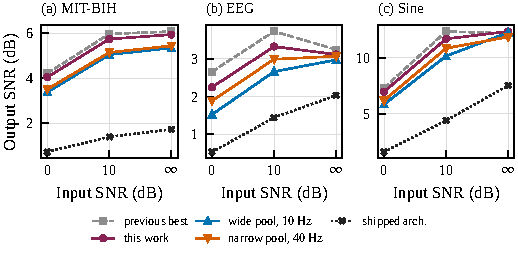
\includegraphics[width=\columnwidth]{fig_noisy.pdf}
\caption{The named designs at noisy inputs (confirmation grid, seeds
10--19): output SNR at 0\dB, 10\dB{} and noiseless input; medians over 16
records (a) or 10 seeds (b, c). D3, the 2-bit D2, is omitted; it lies on D2.}
\label{fig:noisy}
\end{figure}

Realistic sensors are noisy, so the confirmation grid also ran every design at
10\dB{} and 0\dB{} input (Fig.~\ref{fig:noisy}). On MIT-BIH, where the
comparison was tested, D2 stays equivalent to D1 at both inputs, and at 0\dB{}
it delivers 4.04\dB{} against 0.72 for the reference architecture. The
one-layer designs stay far above D0 at every input on all three signals. On
EEG and the sine the headline comparison was tested only at noiseless input,
and there the noisy inputs are less kind: D2's median falls 0.35--0.67\dB{}
below D1's. Some designs on EEG, and D1 on the sine, also score slightly higher
at 10\dB{} input than at a noiseless one. We did not test why; the encoder's
range follows the noisy drive, and on smooth signals that range matters.

Whether D4's saving is real depends on the chip. Writing event cost as
$O + \rho E$ in synaptic-operation equivalents, with $\rho$ the ratio of the
energy of a routed spike to that of a synaptic operation, D4 is cheaper than D5
whenever $\rho < 2.00$ (Fig.~\ref{fig:breakeven}), while D2 is cheaper than D1
at every $\rho$. Across the earlier landscape the cheapest design reaching
5\dB{} changes with $\rho$ (post hoc): the 2048-channel pool at 10~Hz below
$\rho = 0.99$, $[512,128]$ at 20~Hz up to $\rho = 3.25$, and $[128,128]$ with
its layer at 10~Hz above it. The break-even pair holds at clean input only:
with noise, the slower encoder's median ceiling falls 0.10--0.13\dB{} behind on
MIT-BIH and 0.3--0.7\dB{} on EEG and the sine.

\subsection{Weight precision and device faults}
\label{sec:devices}

\begin{figure}[t]
\centering
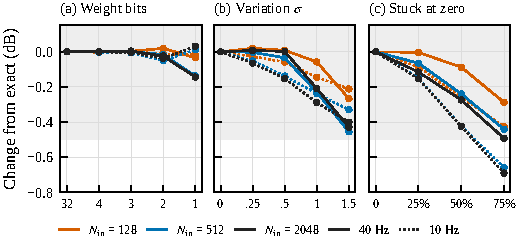
\includegraphics[width=\columnwidth]{fig_devices.pdf}
\caption{Device grid, MIT-BIH, $K = 8$, $N_1 = 128$: change in ceiling from
exact weights against (a) weight bits, (b) lognormal variation and (c) the
fraction of devices stuck at zero, for three pools at 40~Hz (solid) and 10~Hz
(dotted) encoders; medians over 16 records. Shaded: the $\pm0.5$\dB{}
equivalence margin.}
\label{fig:devices}
\end{figure}

\begin{table}[t]
\centering
\caption{Precision and fault budget}
\label{tab:devices}
\scriptsize
\setlength{\tabcolsep}{4pt}
\begin{tabular}{@{}lccc@{}}
\toprule
Device level & Measured (dB) & Predicted (dB) & Equivalent \\
\midrule
1 bit & $-$0.22 to +0.03 & $-$0.51 to $-$0.16 & 9/9 \\
2 bits & $-$0.05 to +0.02 & $-$0.07 to $-$0.02 & 9/9 \\
3 bits & $-$0.01 to 0.00 & $-$0.01 to 0.00 & 9/9 \\
4 bits & 0.00 to 0.00 & 0.00 to 0.00 & 9/9 \\
$\sigma = 0.25$ & $-$0.06 to +0.02 & $-$0.05 to $-$0.01 & 9/9 \\
$\sigma = 0.5$ & $-$0.15 to +0.01 & $-$0.17 to $-$0.05 & 9/9 \\
$\sigma = 1$ & $-$0.29 to $-$0.06 & $-$0.50 to $-$0.15 & 9/9 \\
$\sigma = 1.5$ & $-$0.45 to $-$0.21 & $-$0.80 to $-$0.26 & 5/9 \\
25\% stuck & $-$0.15 to 0.00 & $-$0.35 to $-$0.10 & 9/9 \\
50\% stuck & $-$0.42 to $-$0.09 & $-$0.79 to $-$0.27 & 8/9 \\
75\% stuck & $-$0.69 to $-$0.29 & $-$1.53 to $-$0.61 & 2/9 \\
\bottomrule
\end{tabular}

\vspace{2pt}
\parbox{\columnwidth}{\scriptsize Change from exact weights, range over three pools and three encoder rates (9 points), each a median over 16 records; equivalent: TOST $\pm0.5$~dB. Predicted: effective fan-in model, fixed in advance.}
\end{table}


The device grid asks how much precision and reliability a fixed-fan-in layer
needs (Fig.~\ref{fig:devices}, Table~\ref{tab:devices}). Both budgets set in
advance were met with room to spare. At every pool and encoder rate, 1-bit
weights are equivalent to exact ones, costing at most 0.22\dB, and 2 bits
cost at most 0.05\dB. Lognormal variation is equivalent up to $\sigma = 1.0$ at
all nine points and up to 1.5 at five. Stuck-at-zero devices cost at most
0.15\dB{} at 25\%, 0.42\dB{} at 50\% and 0.69\dB{} at 75\%. Only 12 of the 99
perturbed points fail the equivalence test, seven of them at 75\% stuck.

We also tested whether the budget~\eqref{eq:budget} predicts these losses with
no fitted parameter. Each non-ideality lowers a neuron's effective fan-in, the
participation ratio $(\sum_i w_i)^2/\sum_i w_i^2$, by an amount the weight
matrices give. If the encoder's counting term scaled with its inverse and
$\Lambda_\mathrm{rest}$ stayed put, the losses would follow. The prediction
ranks the losses well (Spearman $\rho_s = 0.81$ over the 99 points, post hoc).
Pairs of levels with matched effective fan-in but two to three times
different spread in each neuron's summed weight are equivalent at all 18
comparisons, so effective fan-in, not heterogeneity, organizes the losses. But
the model overstates their size: measured losses are 0.44 times the predicted
ones (post hoc). On the 22 points predicted to lose at least 0.5\dB{} a
no-change model predicts better, with a median absolute error of 0.37\dB{}
against 0.46\dB, so the test we committed to failed. The model errs most in
narrow pools, and it orders the pools wrongly: it predicts that wide pools lose
less to stuck devices, but they lose more, 0.49\dB{} at 2048 channels against
0.29\dB{} at 128 with 75\% stuck and a 40~Hz encoder. They still end higher,
at 5.19 against 4.84\dB. One reading, untested, is that faults in a narrow pool also thin the
overlap between neurons' inputs, which offsets part of the loss, so
$\Lambda_\mathrm{rest}$ does not in fact stay put.

\section{Discussion}
\label{sec:discussion}

\emph{Design rules.} For rate-coded spiking chains of the kind studied here:
\begin{itemize}
\item Use one spiking layer. A second costs 2.5 times the synaptic work and
0.9\dB.
\item Give each neuron about eight inputs and widen the input pool, not the
layer. Pool width costs spikes, not synaptic operations.
\item Choose the encoder rate from the chip's spike-to-synaptic-operation
energy ratio: \eqref{eq:budget} gives the fidelity side, and
$O + \rho E$ gives the cost side.
\item Store weights in two bits. Budget one bit if 0.22\dB{} is affordable, and
expect a quarter of open devices to cost under 0.2\dB.
\end{itemize}
Together these give Table~\ref{tab:designs}'s D3: six times the S/N of the
reference architecture for 1.6 times its synaptic work, and, through D2,
equivalent to a network with eight times the synaptic work and, at 32-bit
weights, 30 times the weight memory, addresses included.

\emph{Mapping to hardware.} Each term of \eqref{eq:cost} and
\eqref{eq:memory} is a component. The input pool is a bank of $\Nin$
stochastic comparators: at every step each channel compares the normalized
sample with its own random threshold and fires if the sample exceeds it. The
channels need independent random numbers, because the gain from widening the
pool comes from their independent counting noise; we did not test a pool
driven by correlated random streams. The pool emits $\Nin r_0$ address events
per second of $\lceil \log_2 \Nin \rceil$ bits each~\cite{boahen2000aer},
about 20 thousand 9-bit events for D2, and in a clock-driven encoder it also costs
$250\,\Nin$ comparisons per second. A fixed-fan-in layer is a sparse
connectivity table of $K$ address--weight pairs per neuron, 1,024 entries for
D2; a dense crossbar between the same pool and layer would hold 64 times as
many weights. Rate calibration needs one gain per layer, a single register or
bias current, tuned by counting output spikes; the device grid assumes it is
re-tuned after the weights are programmed. On an event-driven core, fan-in and the
encoder rate cut work directly, and a wide pool buys fidelity without adding
synaptic work. On a clock-driven core only the synapse count matters, and a
wide pool adds comparisons.

\emph{What the budget does and does not price.} Equation~\eqref{eq:budget}
prices the encoder: its counting term follows $1/r_0$ to a few hundredths of a
dB. Effective fan-in ranks device losses, but a model that holds the
remainder fixed overstates them. Designers can use the counting term to set
rates, but device budgets should be measured, as in Table~\ref{tab:devices}.

\emph{Limitations.} All results are simulations; we count events and bits and
report no energies, so $\rho$ must come from the target chip. The input pool is
$\Nin$ independent Poisson draws of one signal, which a front end must provide
as independent stochastic encoders. The networks are untrained, feed-forward
and without inhibition, and the device grid assumes one layer gain is
recalibrated after programming. Faults were independent, applied one kind at
a time, and did not include cycle-to-cycle read noise. Every SNR is causal. The
break-even example holds at clean input only. The main grids used one ECG
database, which the confirmation grid supplements with only two synthetic
signals.

\section{Conclusion}

Fidelity in a rate-coded spiking signal chain has a price in synaptic
operations, spikes and weight bits, and most of the price is set by design
choices that cost nothing to change. A single layer whose neurons read eight
inputs from a wide pool, with 2-bit weights, matches the best fidelity we
measured at one eighth of the synaptic work and survives heavy device faults.
A counting term prices the encoder rate, and a break-even ratio says when to
spend spikes to save synaptic operations. Signed weights and on-chip learning
with bounded fan-in are the natural next tests.

\bibliographystyle{IEEEtran}
\bibliography{refs}

\end{document}
